\documentclass[12pt, oneside]{book}

% Pacotes necessários
\usepackage[portuguese]{babel}
\usepackage[utf8]{inputenc}
\usepackage[scale=1.5]{ccicons}
\usepackage{graphicx}
\usepackage{titlesec}
\usepackage{setspace}
\usepackage{geometry}
\usepackage{indentfirst}
\usepackage{hyperref}
\usepackage{float}
\usepackage{tikz}
\usepackage{kpfonts}
\usepackage{fontawesome5}
\usepackage{fancyhdr}
\usepackage{subfigure}
\usepackage{tcolorbox}
\usepackage{xcolor}
\usepackage{pgfplots}

% Define o estilo da página
\pagestyle{fancy}
\fancyhf{}
\fancyfoot[L]{Erick Faria}
\fancyfoot[C]{\thepage}
\fancyfoot[R]{\href{https://www.balaiocientifico.com/}{Balaio Científico}}
\fancyhead[R]{\nouppercase{\leftmark}}
\renewcommand{\headrulewidth}{0.4pt}
\renewcommand{\footrulewidth}{0.4pt}
% Redefine o comando \chaptermark para remover o prefixo "Chapter X."
\renewcommand{\chaptermark}[1]{\markboth{#1}{}}


\usefont{T1}{jkpss}{m}{n}

\geometry{
  left=3cm,
  right=2cm,
  top=3cm,
  bottom=2cm,
  bindingoffset=0cm
}

\onehalfspacing

% Define o caminho das imagens
\graphicspath{{imagens/}}

% Define o estilo de início do capítulo
\titleformat{\chapter}[display]
  {\normalfont\huge\bfseries\filcenter}
  {\begin{tikzpicture}[remember picture,overlay]
    \node[anchor=north west,inner sep=0pt] at (current page.north west)
      {
\includegraphics[width=\paperwidth,height=0.2\paperheight]{imagens/fundo_cap.pdf}};
    \fill[white,opacity=0] (current page.north west) rectangle (current page.south east);
    \draw[anchor=north west] (0.2\paperwidth,0.2\paperheight) node [font=\Huge\bfseries] {\chaptertitlename\ \thechapter};
  \end{tikzpicture}}
  {0pt}
  {\Huge}

% Define os metadados do documento
\hypersetup{
colorlinks=true,
linkcolor=blue,
filecolor=magenta,      
urlcolor=blue,
pdftitle={Apostila de Jamovi},
pdfauthor={Erick Faria},
pdfsubject={Apostila de Jamovi},
pdfkeywords={Jamovi, Estatística, Análise de Dados}
}

\begin{document}
\let\cleardoublepage\clearpage

% Inclui a capa
\begin{titlepage}
	\centering % Center everything on the title page
	\scshape % Use small caps for all text on the title page
	\vspace*{1.5\baselineskip} % White space at the top of the page
% ===================
%	Title Section 	
% ===================

	\rule{13cm}{1.6pt}\vspace*{-\baselineskip}\vspace*{2pt} % Thick horizontal rule
	\rule{13cm}{0.4pt} % Thin horizontal rule
	
		\vspace{0.75\baselineskip} % Whitespace above the title
% ========== Title ===============	
	{	\Huge Introdução ao\\ 
			\vspace{4mm}
		JAMOVI \\	}
% ======================================
		\vspace{0.75\baselineskip} % Whitespace below the title
	\rule{13cm}{0.4pt}\vspace*{-\baselineskip}\vspace{3.2pt} % Thin horizontal rule
	\rule{13cm}{1.6pt} % Thick horizontal rule
	
		\vspace{1.75\baselineskip} % Whitespace after the title block
% =================
%	Information	
% =================
	{\large Produzido por: \href{https://www.balaiocientifico.com/author/erickfaria/}{Erick Faria} \\
		\vspace*{1.2\baselineskip}}
	% \href{mailto:erickfaria@balaiocientifico.com}{erickfaria@balaiocientifico.com}} \\
	\vfill
\url{www.balaiocientifico.com}\\
\vspace{0.5cm}
\ccbyncsa
\end{titlepage}

% Define a numeração das páginas em romanos
\pagenumbering{roman}
\setcounter{page}{1}

% Inclui a página de atribuição
\vfill
\small{\noindent \textbf{Você tem o direito de:} \vspace{-3mm}\\
\noindent \rule{3.3cm}{0.5pt} \\
\textbf{Compartilhar }— copiar e redistribuir o material em qualquer suporte ou formato \\
\textbf{Adaptar} — remixar, transformar, e criar a partir do material \\
\\
\small{\noindent \textbf{De acordo com os termos seguintes:} \vspace{-3mm}\\
\noindent \rule{3.3cm}{0.5pt} \\
\textbf{Atribuição} — Você deve dar o crédito apropriado, prover um link para a licença e indicar se mudanças foram feitas. Você deve fazê-lo em qualquer circunstância razoável, mas de nenhuma maneira que sugira que o licenciante apoia você ou o seu uso.  \\
\textbf{NãoComercial} — Você não pode usar o material para fins comerciais.\\
\textbf{CompartilhaIgual} - Se você remixar, transformar, ou criar a partir do material, tem de distribuir as suas contribuições sob a mesma licença que o original.  \\
\\
\centerline{\href{https://creativecommons.org/licenses/by-nc-sa/4.0/deed.pt_BR}{Atribuição-NãoComercial-CompartilhaIgual 4.0 Internacional (CC BY-NC-SA 4.0)}}\\
\centerline{\ccbyncsa}

% Define o nome do sumário
\renewcommand{\contentsname}{Sumário}

% Inclui o sumário
\tableofcontents

% Define a numeração das páginas em arábicos
\pagenumbering{arabic}
\setcounter{page}{1}

% Inclui o primeiro capítulo
\chapter{Introdução ao Jamovi}

\section{O que é o Jamovi?}

O jamovi é um software estatístico com interface gráfica. É um software relativamente novo, se comparado com os seus concorrentes como o SPSS, SAS e PSPP. Com o jamovi você consegue ter um ambiente de fácil aprendizado e fácil manuseio, pois é possível integrar a facilidade do ambiente gráfico, com o poder da linguagem R para a automação de trabalhos.

Além das análises estatísticas convencionais, tais como: estatística descritiva, tabelas cruzadas, boxplot, etc. É possível desenvolver modelos matemáticos. Assim, podemos definir o jamovi como uma solução completa para análises quantitativas e qualitativas com o uso da matemática e estatística. Um software estatístico completo e gratuito.

\subsection{Um software estatístico completo}

O jamovi é um dos softwares mais completos da atualidade. Sua interface gráfica e a integração com a linguagem de programação R, faz com que o programa seja capaz de realizar todas as análises, das mais simples até as mais importantes

Além de ser completo é um software open source e gratuito. Isso significa que você não precisa se preocupar em comprar licença e/ou fazer assinaturas. Além de ser gratuito, o fato de os códigos serem abertos, permite que todos e todas possam verificar diretamente no código fonte como o programa foi escrito, trazendo mais transparência e segurança para os(as) usuários(as)

\subsection{Estatística com interface gráfica}

Uma das principais barreiras para várias pessoas que desejam estudar estatística é a programação. Geralmente os(as) alunos(as) que estão começando a estudar estatística, estão começando também a ter o primeiro contato com a linguagem de programação

Uma das principais vantagens do Jamovi é sua interface gráfica. Com ela, o(a) aluno(a) que está começando nos estudos de estatística, pode se concentrar apenas no estudo teórico, deixando para outro momento o estudo da programação. Dessa forma, o jamovi é uma das melhores alternativas de software para estudos em estatística, pois permite que o(a) aluno(a) possa ver os resultados em tempo real, sem a necessidade de aprender os comandos de uma linguagem

\subsection{Software Modular}

O jamovi é um software modular. Isso significa que você pode instalar complementos, ou módulos de acordo com a sua necessidade. Diferentemente do SPSS, por exemplo, com o Jamovi você tem a liberdade de instalar somente os módulos que você precisa; algo que não é possível fazer no SPSS.

A liberdade de poder instalar os módulos, faz do Jamovi um software leve e personalizável. Além disso, a comunidade está ativamente desenvolvendo novos módulos, o que faz com que o Jamovi seja cada vez mais completo e flexível para atender diversos usuários

\subsection{Ambiente para aprender a linguagem R}

Apesar de ser um software com interface gráfica, o Jamovi tem integração com a linguagem de programação R. Isso significa que você tem a facilidade da interface gráfica, com o poder e a flexibilidade de uma das linguagens mais utilizadas no mundo da estatística.

Caso o Jamovi não tenha nativamente uma função que você precisa, você pode desenvolver utilizando a linguagem R. Essa integração faz com que seja possível realizar qualquer tipo de análise com o Jamovi. Além disso, você pode automatizar rotinas que são repetitivas e você precisa realizar várias vezes no seu trabalho e estudo.

\begin{tcolorbox}[colback=white,colframe=green!50!black,title= Dica de Conteúdo]
  Preparei um vídeo super especial de introdução ao jamovi, que vai te ajudar a dar os primeiros passos nessa incrível ferramenta estatística. Depois de ler a seção da apostila, não deixe de conferir essa videoaula, tenho certeza de que você vai adorar e aprender muito. Clique no link abaixo e aproveite!\\
  \faYoutube{} \href{https://www.youtube.com/watch?v=0zGH20Fa_JA&t=2s}{Introdução ao Jamovi}
\end{tcolorbox}

\section{Instalação do Jamovi}

Para fazer a instalação do software Jamovi, é muito simples e dependerá apenas do sistema operacional em que você está utilizando.

Se você fizer a instalação no site oficial você não precisa se preocupar com a sua segurança e está livre para instalar e fazer o uso do programa da forma que você precisar. Não existe nenhum tipo de restrição quanto ao uso ou locais em que você deve instalar.

Assim, você é livre para fazer uso educacional, comercial ou qualquer outro motivo pois não há nenhum tipo de restrição quanto ao uso ou a licença do programa.

\subsection{Download do Jamovi}

Para você fazer a utilização do jamovi, existem duas possibilidades: uma em cloud sendo que você não precisa realizar nenhum tipo de instalação e pode utilizar o programa diretamente da internet; em uma opção localmente em que você pode fazer o download no seu computador e instalar como um programa qualquer.

As duas soluções são muito boas, entretanto eu aconselho que você faça a instalação no seu computador para que você tenha total controle sobre os dados e não corra o risco de perder dados na solução de nuvem.

Eu recomendo que você faça a utilização do programa em nuvem somente em casos em que você não tem a possibilidade de instalar o jamovi em seu computador.

Nas duas sessões posteriores vou ensinar para vocês um pouco de como prosseguir para fazer a utilização das duas formas.

\subsection{Jamovi para desktop}

Primeiramente é importante que você acesse a página oficial do Jamovi para fazer o download. Você pode acessá-la na seguinte página: \url{https://www.jamovi.org}. É fortemente aconselhável que você faça o download somente na página oficial. Vale lembrar que o Jamovi é gratuito e não é necessário recorrer e nenhum programa paralelo, ou site diferente do oficial.

Para fazer a instalação em seu computador você deve selecionar a opção correspondente para instalação no desktop. No momento em que eu preparo esse material o site está organizado da seguinte forma.

Ao entrar na parte de download você verá uma página como na figura \ref{fig:download_jamovi}.

\begin{figure}[H]
  \centering
  \caption{Opção de Download do Jamovi para Desktop}
  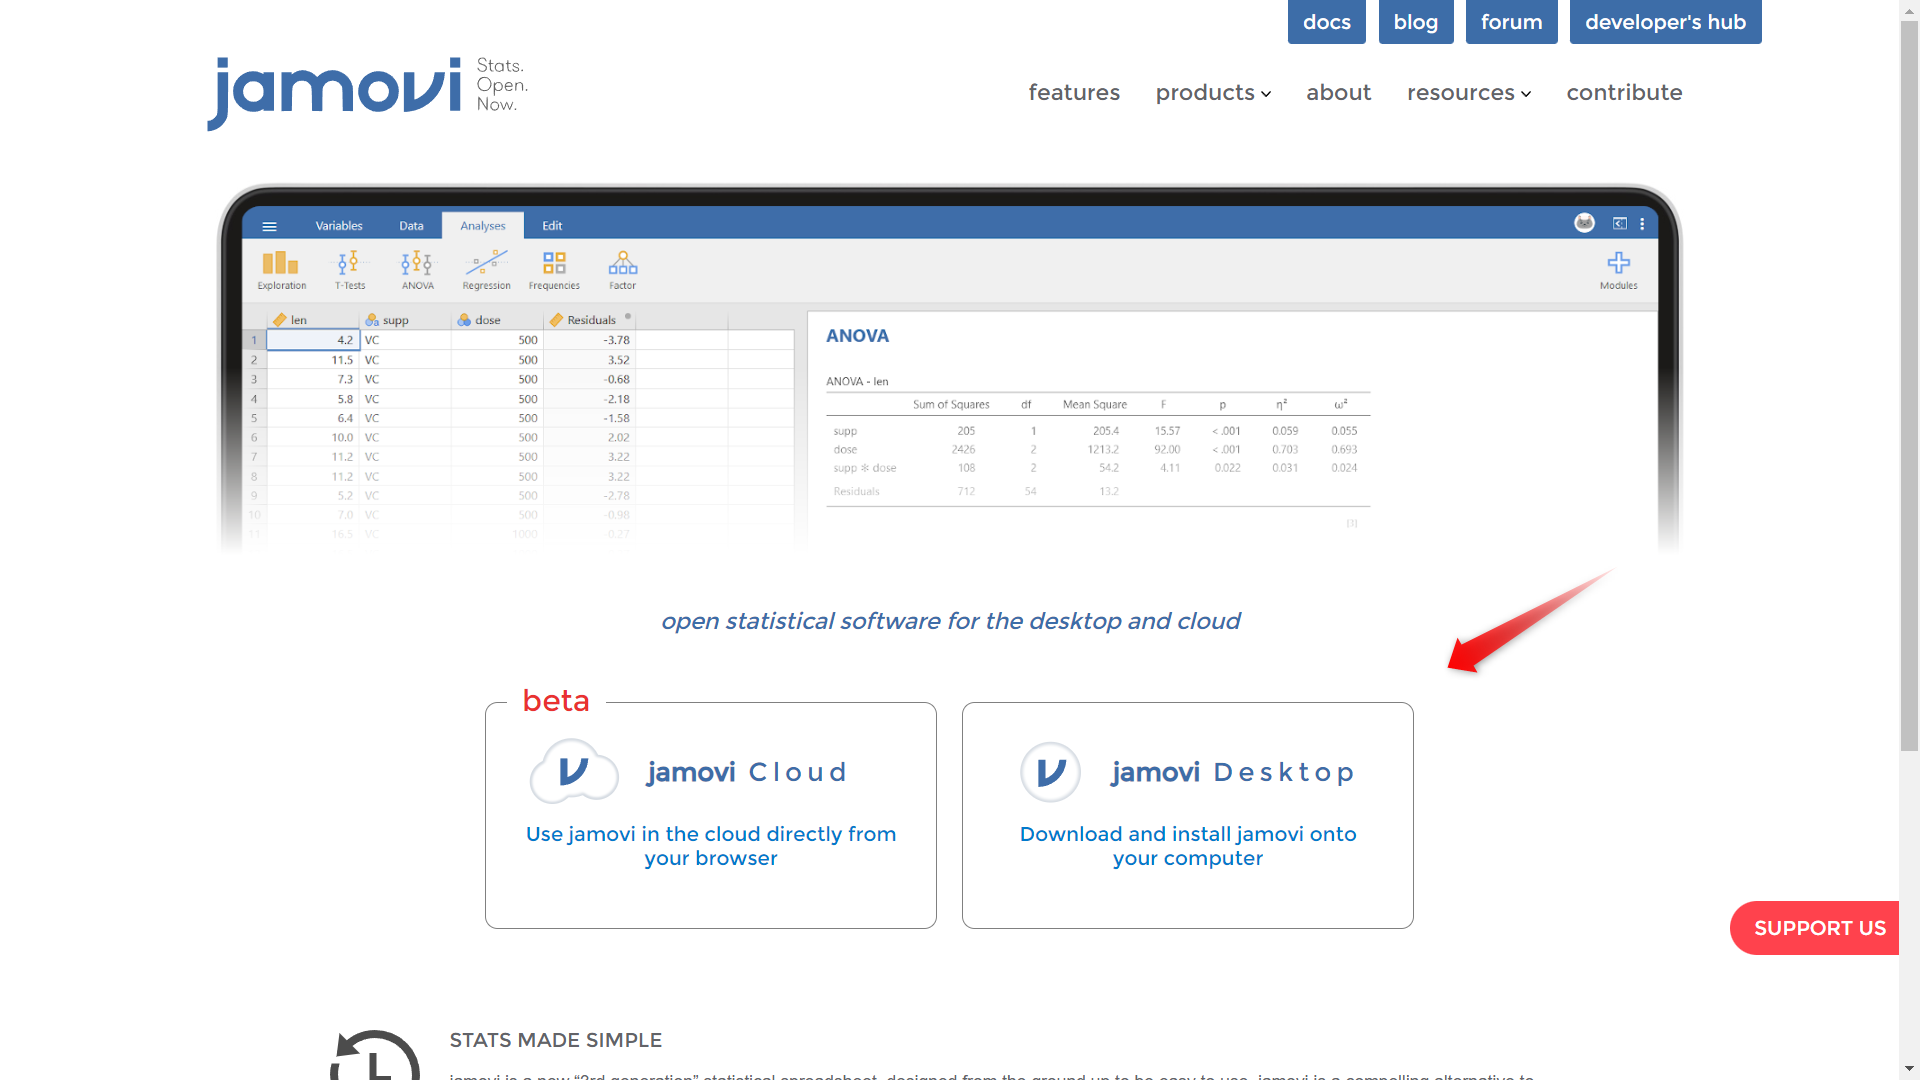
\includegraphics[width=\textwidth]{imagens/cap_1/download_jamovi.png}
  \label{fig:download_jamovi}
\end{figure}

Selecione a opção desktop conforme indicado na imagem \ref{fig:download_jamovi} com uma seta. Ao clicar avance para o próximo tópico da apostila, pois vamos selecionar a versão do Jamovi que será instalada.

\subsection{Selecionando a versão do Jamovi}

Para fazer o download do Jamovi em seu computador, você precisa selecionar a versão correspondente ao seu sistema operacional. É importante que você faça a escolha correta, pois caso você cometa um equívoco na escola o programa não funcionará, ou não funcionará corretamente.

Geralmente quando você chegar na página de download, o próprio site já irá indicar a versão correta, correspondente ao seu sistema operacional. Basta você conferir e prosseguir para o download do programa.

Caso a sugestão do site esteja errada, basta rolar a página um pouco para baixo e selecionar a versão correta correspondente, assim como mostrado na imagem abaixo.

\begin{figure}[H]
  \centering
  \caption{Seleciona a versão do Jamovi}
  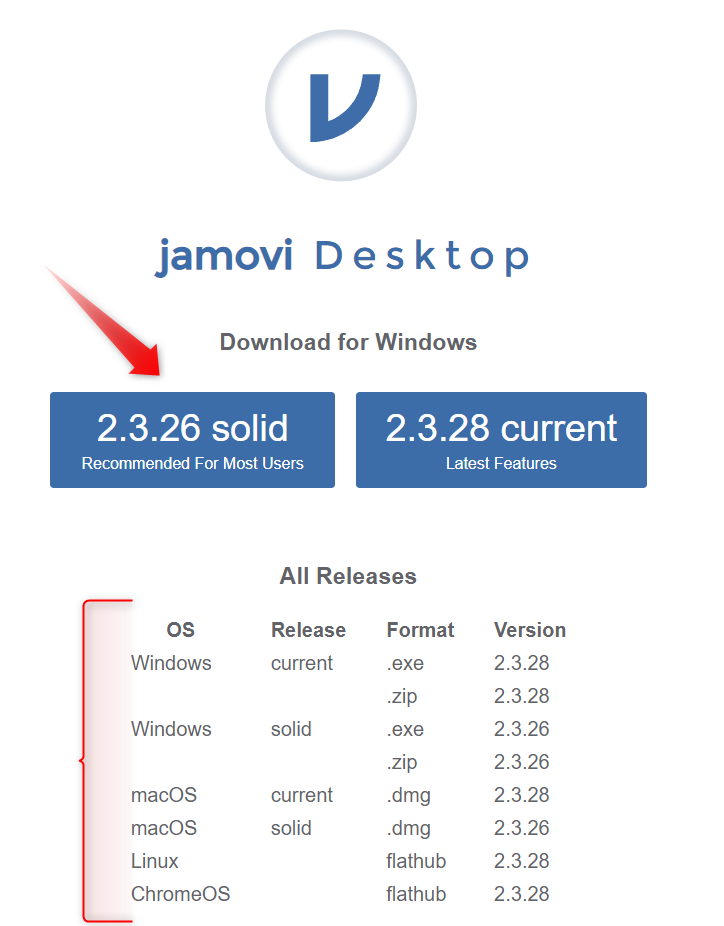
\includegraphics[width=0.5\textwidth]{imagens/cap_1/seleciona_versao_jamovi.png}
  \label{fig:download_jamovi}
\end{figure}

Quando você selecionar a versão que deseja utilizar, o download irá iniciar automaticamente.

\section{Instalando o Jamovi}

Após fazer o download do Jamovi, chegou o momento de você fazer a instalação em seu computador. Clique no arquivo que você acabou de baixar e siga as instuções para instalação.

O processo de instalação é simples e segue o mesmo fluxo de qualquer programa que você já está habituado(a) a fazer. Basta ir clicando em prosseguir, indicar um caminho de instalação, caso você queira selecionar uma pasta diferente dá pasta padrão e concluir a instalação.

\subsection{Jamovi em nuvem – cloud}

Na versão cloud você deve selecionar a opção correspondente como apontado na imagem \ref{fig:jamovi-cloud}.

\begin{figure}[H]
  \centering
  \caption{Versão cloud do Jamovi}
  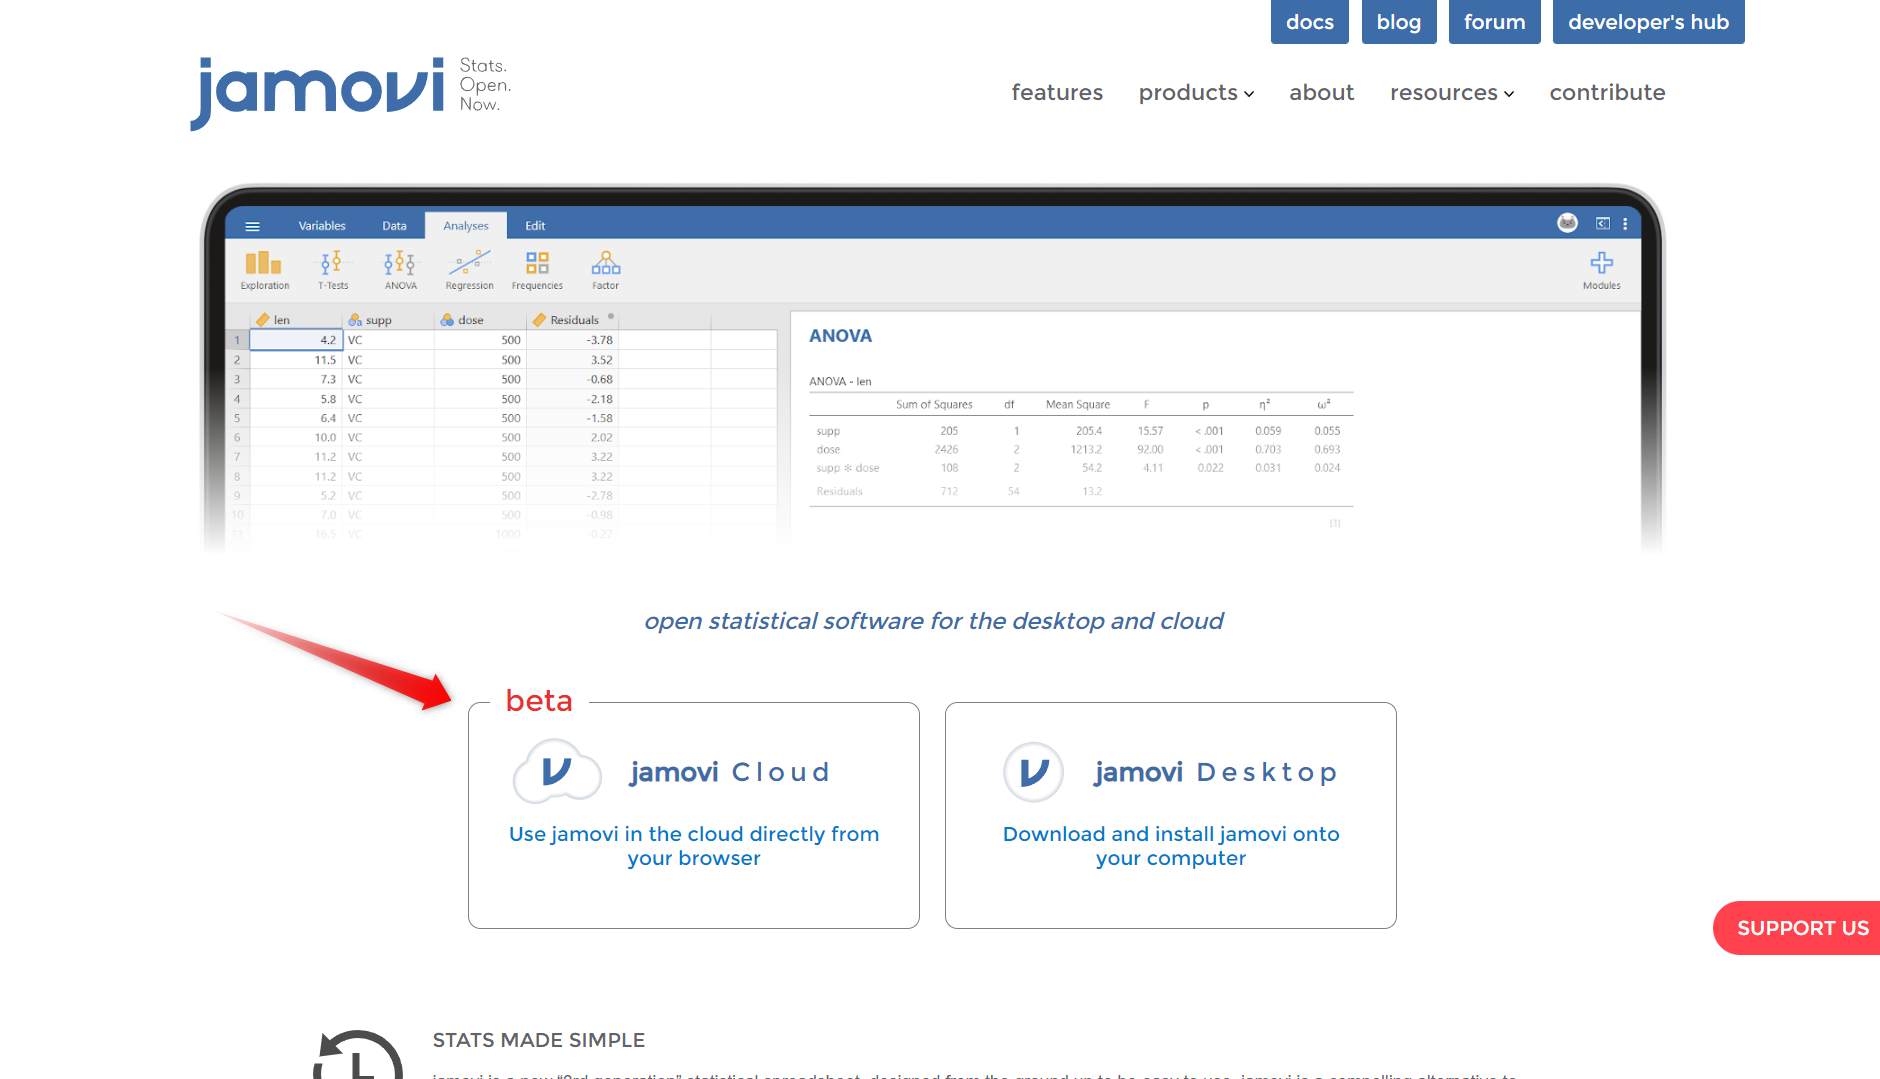
\includegraphics[width=\textwidth]{imagens/cap_1/jamovi-cloud.png}
  \label{fig:jamovi-cloud}
\end{figure}

Ao clicar na versão cloud você irá se deparar com duas opções de utilização. Uma gratuita e outra paga.

Cabe você decidir se vale a pena pagar ou não para utilizar o Jamovi em cloud. A diferença da versão paga para a gratuita é apenas nos recursos computacionais e na disponibilidade do servidor onde o Jamovi é executado.

Entenda que executar um software em nuvem requer a utilização de infraestrutura e se um programa está sendo executado e não é em seu computador, algum lugar está fazendo para você.

Veja na imagem abaixo as opções que você pode escolher:

\begin{figure}[H]
  \centering
  \caption{Opções de utilização do Jamovi em cloud}
  
\includegraphics[width=0.5\textwidth]{imagens/cap_1/opcoes_cloud.png}
  \label{fig:jamovi-cloud}
\end{figure}

Eu sou um grande entusiasta das soluções que são executadas em nuvem. Quase todos os meus trabalhos eu faço questão de utilizar algumas soluções em nuvem para realizar.

Caso eu fizesse o uso intensivo do jamovi em algum projeto meu, eu faria a assinatura sem problema. Entretanto se você é um estudante e não tem muitos recursos para fazer uma assinatura nesse momento, use a versão gratuita para realizar os seus estudos ou então ignore essa opção de utilização em nuvem e faça a utilização do programa instalando em seu computador normalmente.

Caso um dia você veja que faz sentido para você fazer assinatura para utilizar em algum projeto específico você vem faz a assinatura e faz a utilização normalmente. Assim, quando você for utilizar você já será um usuário avançado e poderá tirar todos os benefícios da solução em nuvem.

\section{Primeiros passos com o Jamovi}

Ao abrir o Jamovi pela primeira vez em seu computador, você verá uma imagem semelhante a esta mostrada abaixo. Essa é a interface gráfica do Jamovi e é onde você verá os dados e gráficos.

\begin{figure}[H]
  \centering
  \caption{Captura de Tela do Jamovi}
  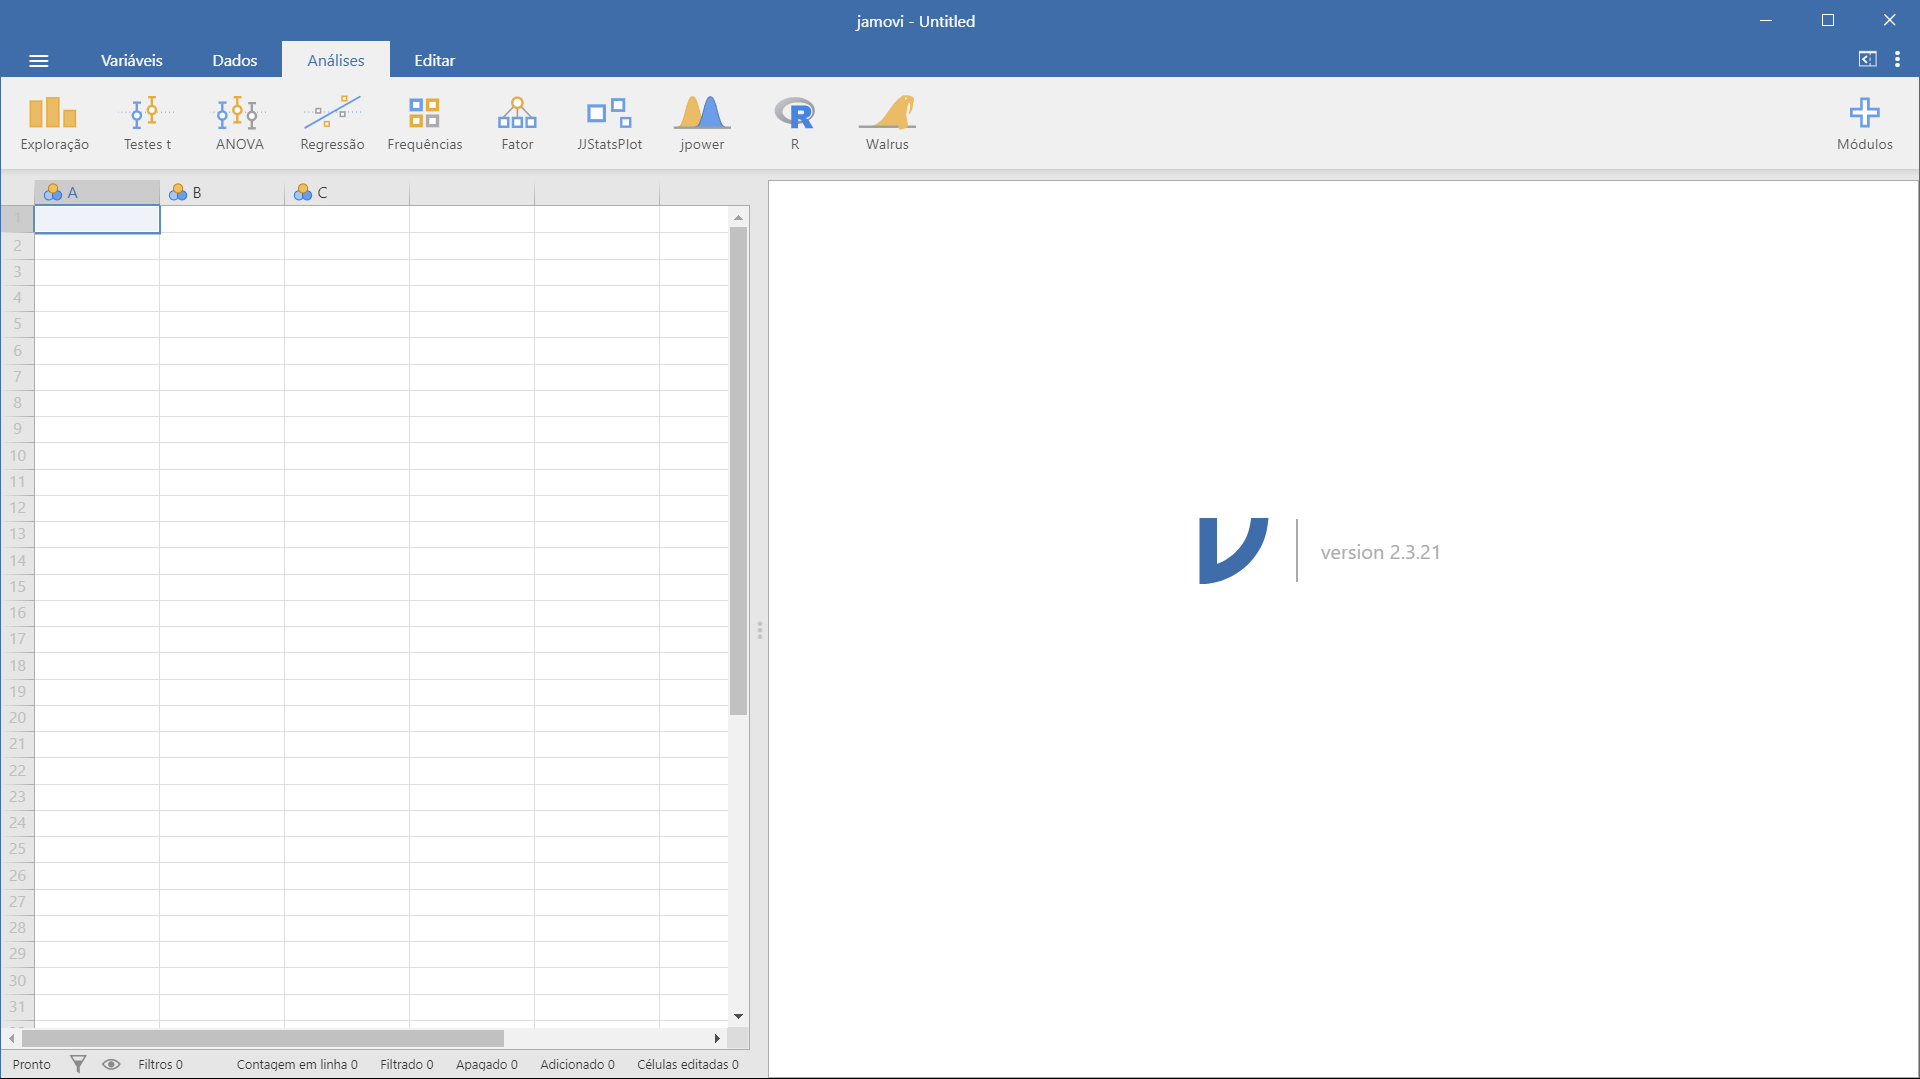
\includegraphics[width=\textwidth]{imagens/cap_1/captura_tela_jamovi.png}
  \label{fig:captura_tela_jamovi}
\end{figure}

\begin{tcolorbox}[colback=white,colframe=green!50!black,title= Dica de Conteúdo]
  Se você encontrou dificuldades nessa etapa, não se preocupe. Assista a videoaula a seguir em que eu ensino como dar os primeiros passos com o Jamovi. Nessa videoaula você será capaz de ver com maior clareza as etapas para iniciar no Jamovi.\\
  \faYoutube{} \href{https://www.youtube.com/watch?v=bV9hlHPLe5I&t=5s}{Primeiros Passos}
\end{tcolorbox}

\subsection{Importando dados no Jamovi}

Neste momento, é chegada a hora de realizar a leitura dos dados no Jamovi. Esse processo é conhecido por diversos termos, como importação, leitura ou carregamento de dados no software. Particularmente, opto por utilizar o termo importação de dados no Jamovi, embora seja válido utilizar a denominação de sua preferência.

Nessa seção eu vou utilizar os dados de passageiros do titanic como exemplo para ensinar a importação de dados do jamovi. Caso você tenha interesse de utilizar o mesmo conjunto de dados que eu, basta fazer o download do arquivo csv no \href{https://github.com/balaio-cientifico/dataset}{repositório oficial do Balaio Científico}.

Com o Jamovi aberto, acesse o menu principal do software clicando no ícone localizado no canto superior esquerdo da tela. Ao realizar essa ação, uma nova janela será exibida. Observe a imagem abaixo para identificar o ícone a ser selecionado, indicado pela seta.

\begin{figure}[H]
  \centering
  \caption{Captura de Tela do Jamovi}
  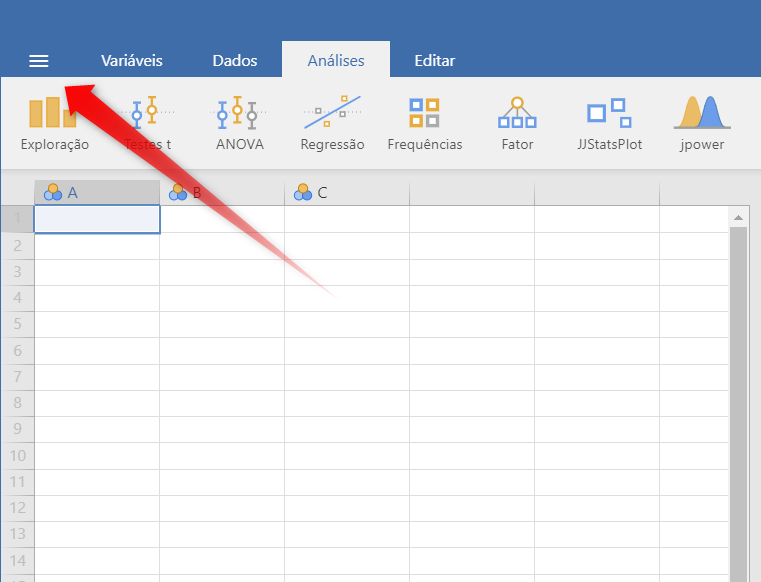
\includegraphics[width=\textwidth]{imagens/cap_1/importa_dados_1.png}
  \label{fig:importa_dados_1}
\end{figure}

Após clicar em “Abrir”, selecione a opção “Este PC”. No exemplo apresentado, alguns arquivos que já foram abertos anteriormente são exibidos. Entretanto, se este for o primeiro uso do Jamovi, é necessário clicar em “Procurar” e navegar até o local em que o arquivo de interesse está salvo para, então, importá-lo no software. Para localizar o arquivo, basta navegar pelas pastas até encontrar o diretório em que o arquivo está armazenado.

\begin{figure}[H]
  \centering
  \caption{Captura de Tela do Jamovi}
  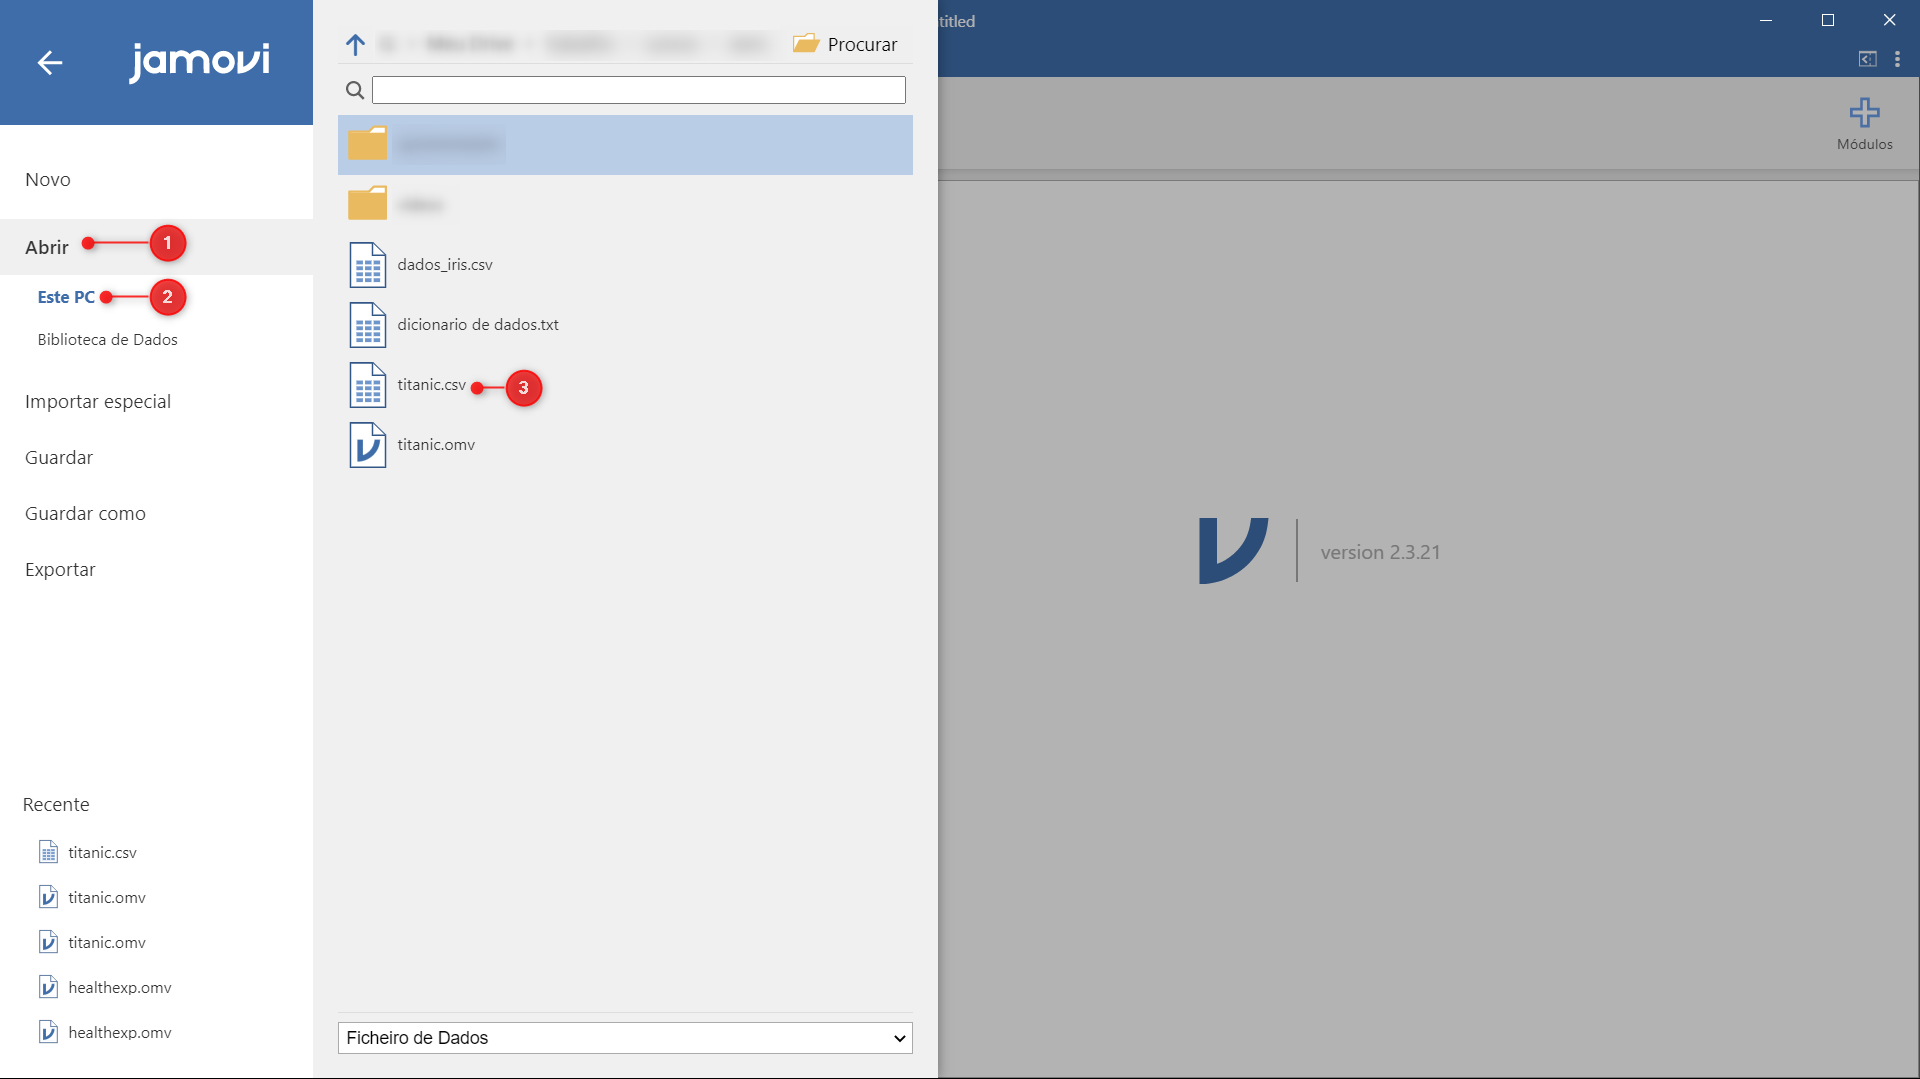
\includegraphics[width=\textwidth]{imagens/cap_1/importa_dados_2.png}
  \label{fig:importa_dados_2}
\end{figure}

Ao clicar no arquivo que contém o conjunto de dados, o Jamovi realizará automaticamente a configuração e importação dos dados. Se você tiver importado os mesmos dados do exemplo apresentado, uma janela semelhante à imagem abaixo será exibida.

\begin{figure}[H]
  \centering
  \caption{Captura de Tela do Jamovi}
  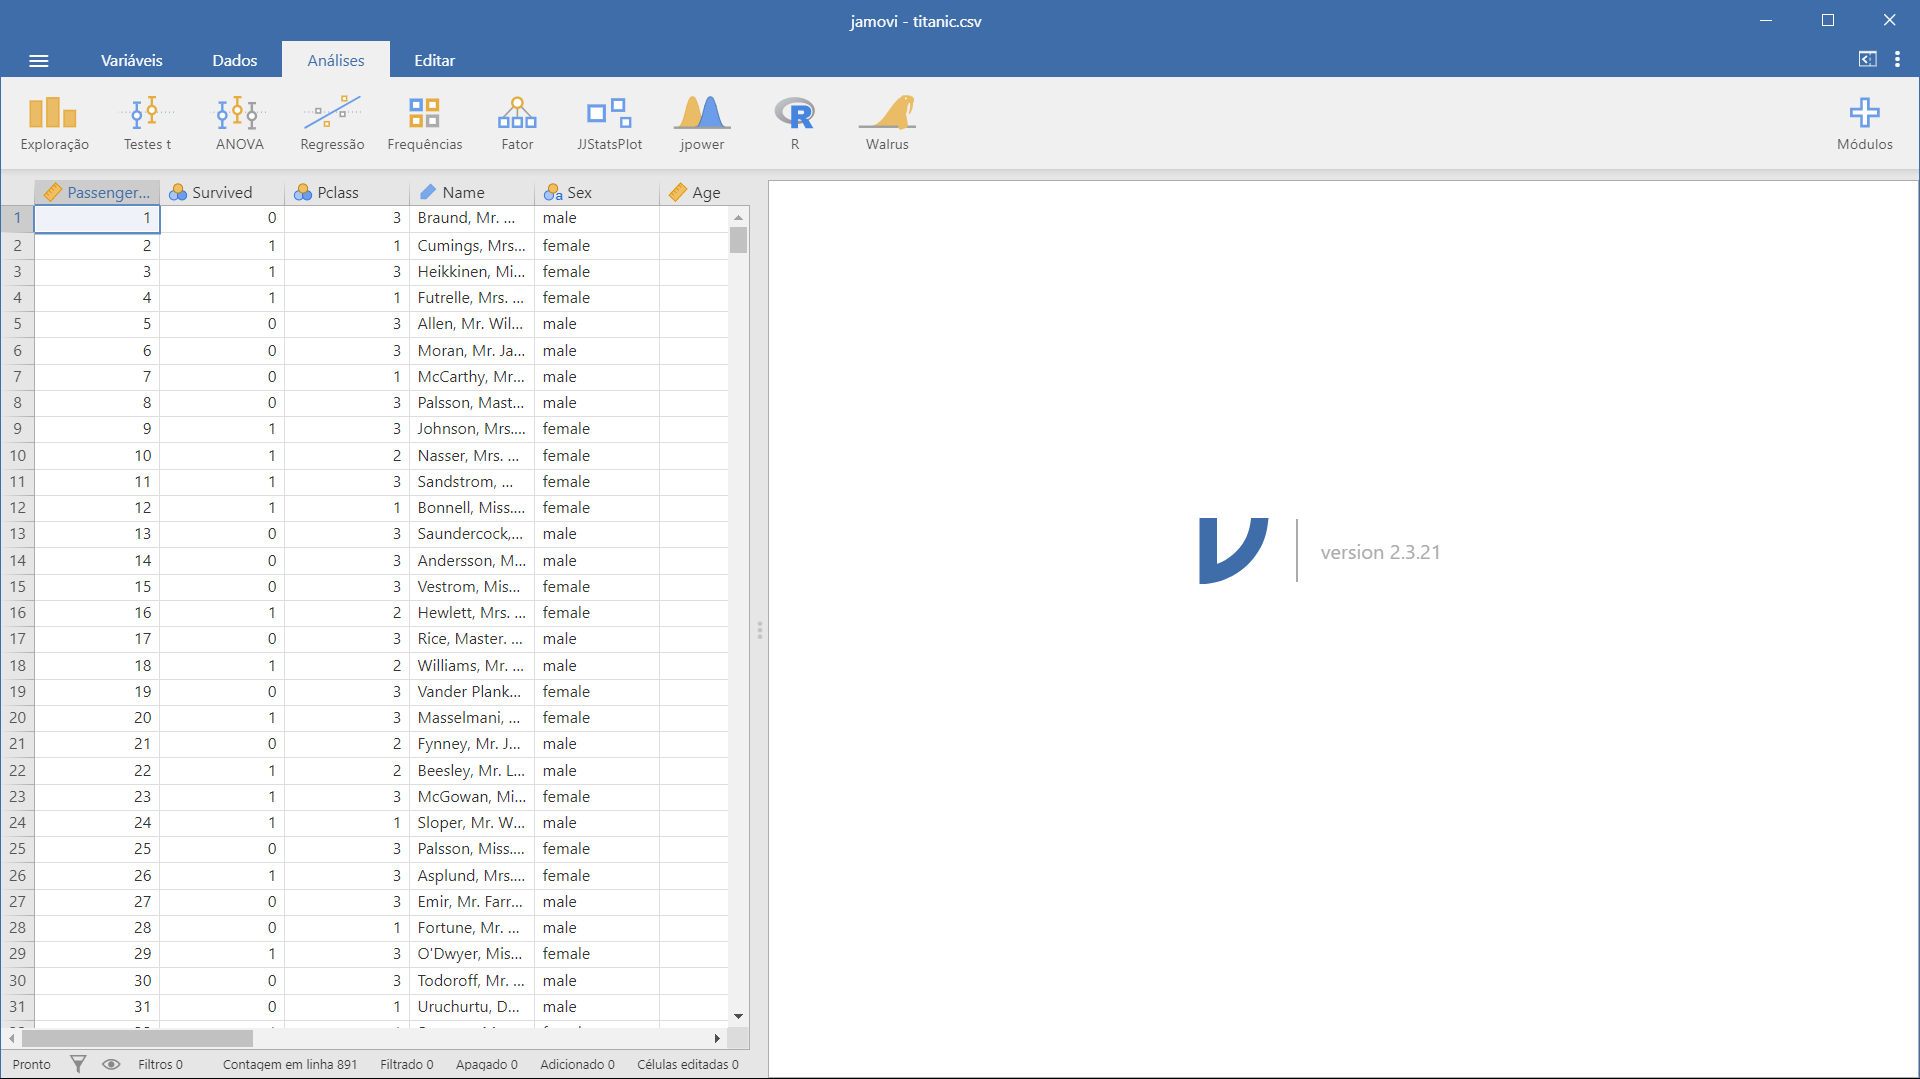
\includegraphics[width=\textwidth]{imagens/cap_1/jamovi_arquivo_importado.png}
  \label{fig:jamovi_arquivo_importado}
\end{figure}

Após a importação dos dados, você estará pronto(a) para começar a realizar análises estatísticas e utilizar todas as funcionalidades disponíveis no Jamovi. É importante praticar a importação de diferentes conjuntos de dados para se familiarizar com o processo e estar apto(a) a realizá-lo com facilidade.

\begin{tcolorbox}[colback=white,colframe=green!50!black,title= Dica de Conteúdo]
  Se você teve dificuldades para fazer a importação dos dados não se preocupe. Essa video aula vai te mostrarcom todos os detalhes como você pode fazer a importação dos dados do Jamovi. Destaco que essa é uma das etapas mais importantes, logo tenha certeza de que entendeu corretamente para que seu aprendizado não fique prejudicado.\\
  \faYoutube{} \href{https://www.youtube.com/watch?v=NIpt0wIq5pc&t=1s}{Importar Dados no Jamovi}
\end{tcolorbox}
\chapter{Estatística Descritiva}

A estatística descritiva no Jamovi é uma técnica utilizada para organizar, resumir e apresentar dados de forma clara e concisa. Ela é utilizada para descrever as características dos dados, como a média, mediana, moda, desvio padrão, frequência, entre outros.

No Jamovi, é possível acessar várias ferramentas para realizar estatística descritiva, como gráficos, tabelas e estatísticas básicas. Ele também permite que você crie tabelas cruzadas, boxplots e histogramas para visualizar os dados de forma mais fácil. Além disso, o Jamovi também permite a criação de relatórios de estatísticas descritivas para compartilhar com outros pesquisadores.

\faYoutube{}
\chapter{Testes de Hipóteses}

Os testes de hipóteses são ferramentas fundamentais na área da estatística para auxiliar na tomada de decisões baseadas em evidências empíricas. Esses testes permitem que os pesquisadores avaliem se uma determinada afirmação sobre uma população, chamada de hipótese, é consistente com os dados observados.

Em um teste de hipóteses, temos duas hipóteses a serem consideradas: a hipótese nula (H0) e a hipótese alternativa (H1). A hipótese nula é a afirmação que queremos testar, enquanto a hipótese alternativa é a afirmação oposta à hipótese nula.

O procedimento envolve coletar dados da população em estudo e realizar cálculos estatísticos com base nessas informações. O objetivo é obter um valor chamado estatística de teste, que fornece uma medida da força das evidências em relação à hipótese nula. Com base nesse valor, é possível calcular o valor p, que representa a probabilidade de obter uma estatística de teste igual ou mais extrema do que a observada, assumindo que a hipótese nula seja verdadeira.

Com base no valor p, os pesquisadores podem tomar uma decisão estatística. Se o valor p for menor do que um nível de significância predefinido, geralmente 0,05, rejeita-se a hipótese nula em favor da hipótese alternativa, indicando que os dados fornecem evidências suficientes para afirmar que a hipótese alternativa é verdadeira. Caso contrário, se o valor p for maior do que o nível de significância, não há evidências suficientes para rejeitar a hipótese nula.

Os testes de hipóteses desempenham um papel importante na pesquisa científica, permitindo que os pesquisadores realizem inferências estatísticas sobre as características de uma população com base em uma amostra limitada de dados. Esses testes fornecem uma estrutura rigorosa para a análise e interpretação dos resultados, contribuindo para a objetividade e a robustez das conclusões estatísticas.
\chapter{Análise de Variância (ANOVA)}

A Análise de Variância (ANOVA) é uma técnica estatística utilizada para comparar as médias de três ou mais grupos independentes. Ela permite determinar se as diferenças observadas entre as médias dos grupos são estatisticamente significativas ou se podem ser atribuídas ao acaso.

A ANOVA baseia-se na decomposição da variabilidade total dos dados em duas componentes: a variabilidade entre os grupos e a variabilidade dentro dos grupos. A ideia fundamental por trás da ANOVA é que, se as médias dos grupos são iguais e as variabilidades dentro dos grupos são semelhantes, então qualquer diferença observada entre as médias pode ser atribuída ao acaso. Por outro lado, se as médias dos grupos são diferentes e/ou as variabilidades dentro dos grupos são grandes em relação à variabilidade entre os grupos, então é mais provável que as diferenças observadas sejam estatisticamente significativas.

Na ANOVA, a hipótese nula assume que não há diferenças entre as médias dos grupos, enquanto a hipótese alternativa considera que pelo menos uma das médias é diferente das demais. O teste estatístico da ANOVA utiliza a estatística F, que compara a variabilidade entre os grupos com a variabilidade dentro dos grupos. Se a estatística F é grande o suficiente para rejeitar a hipótese nula, isso indica que pelo menos uma das médias é estatisticamente diferente das demais.

Existem diferentes tipos de ANOVA, dependendo do design do estudo e do número de fatores considerados. A ANOVA de um fator compara as médias de três ou mais grupos independentes, enquanto a ANOVA de dois fatores analisa o efeito de duas variáveis independentes nos grupos. Além disso, a ANOVA pode ser aplicada em diferentes contextos, como experimentos controlados, estudos observacionais ou análise de dados de pesquisas.

A ANOVA é amplamente utilizada em diversas áreas, como ciências sociais, ciências da saúde, ciências naturais e engenharia. Ela fornece uma abordagem estatística robusta para a comparação de médias de vários grupos, permitindo que os pesquisadores determinem se as diferenças observadas são estatisticamente significativas. A ANOVA também permite realizar análises post hoc para identificar quais grupos diferem significativamente entre si, contribuindo para uma compreensão mais aprofundada dos padrões e relações presentes nos dados.
\chapter{Regressão Linear}

A regressão linear é uma técnica estatística que estuda e modela a relação entre uma variável dependente (ou resposta) e uma ou mais variáveis independentes (ou preditoras). É amplamente utilizada para prever ou estimar o valor de uma variável dependente com base nos valores conhecidos ou observados das variáveis independentes.

Na regressão linear, a relação entre as variáveis é representada por uma equação linear, que é uma linha reta no caso de uma regressão linear simples com uma variável independente, ou um hiperplano em regressões lineares múltiplas com mais de uma variável independente. A equação linear estima a relação entre as variáveis, permitindo fazer previsões ou inferências sobre o comportamento da variável dependente em função das variáveis independentes.

O objetivo da regressão linear é encontrar os coeficientes da equação linear que melhor se ajustem aos dados. Isso é feito por meio de técnicas de otimização que minimizam a diferença entre os valores previstos pela equação linear e os valores observados dos dados. O coeficiente de inclinação (ou declive) da linha ou hiperplano indica a taxa de mudança da variável dependente para cada unidade de mudança nas variáveis independentes, enquanto o coeficiente de interceptação representa o valor estimado da variável dependente quando todas as variáveis independentes são iguais a zero.

A regressão linear é usada em uma ampla gama de aplicações, desde previsão de vendas e análise de mercado até estudos científicos e análise de dados em ciências sociais. Ela permite examinar e quantificar as relações entre variáveis, identificar tendências e padrões nos dados, e fornecer insights úteis para tomadas de decisão e planejamento.

É importante ressaltar que a regressão linear pressupõe uma relação linear entre as variáveis, e sua eficácia depende da validade dessas suposições. Além disso, existem outras variantes da regressão linear, como regressão linear múltipla, regressão linear ponderada e regressão linear não linear, que permitem lidar com casos mais complexos e não lineares.
\chapter{Regressão Linear}

A regressão linear é uma técnica estatística que estuda e modela a relação entre uma variável dependente (ou resposta) e uma ou mais variáveis independentes (ou preditoras). É amplamente utilizada para prever ou estimar o valor de uma variável dependente com base nos valores conhecidos ou observados das variáveis independentes \parencite{Bussab2017}.

Na regressão linear, a relação entre as variáveis é representada por uma equação linear, que é uma linha reta no caso de uma regressão linear simples com uma variável independente, ou um hiperplano em regressões lineares múltiplas com mais de uma variável independente. A equação linear estima a relação entre as variáveis, permitindo fazer previsões ou inferências sobre o comportamento da variável dependente em função das variáveis independentes.

O objetivo da regressão linear é encontrar os coeficientes da equação linear que melhor se ajustem aos dados. Isso é feito por meio de técnicas de otimização que minimizam a diferença entre os valores previstos pela equação linear e os valores observados dos dados. O coeficiente de inclinação (ou declive) da linha ou hiperplano indica a taxa de mudança da variável dependente para cada unidade de mudança nas variáveis independentes, enquanto o coeficiente de interceptação representa o valor estimado da variável dependente quando todas as variáveis independentes são iguais a zero.

A regressão linear é usada em uma ampla gama de aplicações, desde previsão de vendas e análise de mercado até estudos científicos e análise de dados em ciências sociais. Ela permite examinar e quantificar as relações entre variáveis, identificar tendências e padrões nos dados, e fornecer insights úteis para tomadas de decisão e planejamento.

É importante ressaltar que a regressão linear pressupõe uma relação linear entre as variáveis, e sua eficácia depende da validade dessas suposições. Além disso, existem outras variantes da regressão linear, como regressão linear múltipla, regressão linear ponderada e regressão linear não linear, que permitem lidar com casos mais complexos e não lineares.

% Define o final do documento
\backmatter

\end{document}